\chapter{Methodology}\label{methodology}


Each Water Utility is a Client, and the Product is the Application (the \gls{dss}) that the Company (SCUBIC) provides as a cloud-based service. In this chapter, the old architecture of the Application is explained, its flaws are exposed and possible solutions are analyzed. This allows a new, proposed, architecture to be created, one that corrects those flaws.

\section{The Application}\label{methodology:s:the-aplication}

The software that the Company provides to each Client allows the Client's water operators and managers --- the Users --- to access multiple application modules:

\begin{itemize}
    \item Monitoring Module, where data from the Client's sensors can be consulted using charts and other visualization methods. This is the base module, necessary for using the other modules.
    \item Forecasting Module, which performs machine learning operations using the Client's historical sensor data and forecasted weather data to forecast water consumption for the next 24 hours after execution.
    \item Forecasting Model Training Module, which trains the machine-learning models used in the Forecasting Module.
    \item Optimization Module, which relies on the Client's sensor data, forecasted water consumption data and the Simulation submodule to optimize the pump operation schedule for lower operational cost. By optimizing the pumping operation, water and energy usage efficiency increase, lowering CO\textsuperscript{2} emissions and reducing the cost to operate the pumps.
    \item Simulation Module, where a \textit{Smart Digital Twin} of the Client's water network is created and its water pump operations simulated.
    \item \gls{kpi} Module, which performs arithmetic calculations to generate \gls{kpi} regarding the Client's operation.
    \item Solar Forecasting Module, which forecasts photovoltaic solar panel power production for use in conjunction with the Optimization Module.
\end{itemize}  
    
By using the Application's Monitoring Module, each User can access the data generated by the modules (if hired by the Client). 

For these modules to work, each Client is required to send their sensor data, with adequate frequency. Depending on the sensors, this data can be collected by the Client's sensors from every minute up to every hour, which is not synonymous with the data intake frequency. There are Clients who have sensors in remote locations which log data in 15 minute intervals, but due to power constraints this data is only sent once or twice a day to the Client's central monitoring system. Thus, the distinction between data intake frequency and data frequency must be made: the first is related to the frequency with which the sensor data packages arrive at the Application and the latter, the frequency or the time interval between each point of data in the set of sensor data. While the first is important for proper scheduling of the forecasting and optimization tasks performed by the Application, the latter is crucial and needs to have a frequency of up to 1 hour. 

Once data is sent from the Client's databases and to the Application, the data is pre-processed and stored in a time-series\footnote{Series of data points indexed in time order}\label{foot:timeseries} database. The modules access this time-series data in order to perform their tasks. 

These Forecasting, Optimization and Simulation, Solar Forecasting and KPI calculation tasks are performed with a frequency ranging from 8 to 24 hours, every day. For most clients, these tasks are performed once a day, at midnight, in order to prepare the next day's operations. The duration of said tasks can vary, depending on the amount of water consumption points to forecast, the complexity of the water network or on the amount of sensor data to process. These tasks perform calculations using medium-to-large time-series datasets and utilize machine-learning algorithms or complex optimization algorithms in conjunction with water network simulation algorithms. Thus, these tasks are run asynchronously, in \textit{Python} workers.



\section{The Old Architecture}\label{methodology:s:the-old-architecture}

The old software architecture is still in use as of the date of publication of this body of work, alongside the proposed new architecture. They are both in production, with older clients using the old architecture and new clients using the new architecture. \begin{figure}[!htbp]
    \centering
    
\includegraphics[width=0.90\textwidth]{img/diagrams/pdf/old-arch-overview.drawio.pdf}
    \caption[AWS VPC Overview]{The AWS VPC used, hosting the old architecture's EC2 \gls{vps}.}
    \label{fig:old-arch-overview}
\end{figure}
     

\subsection{Overview}\label{methodology:ss:overview}

The old architecture is composed of a group of \gls{ec2} instances, one for each Client, inside the Company's \gls{vpc}. Inside each \gls{ec2} instance, using Docker\footnote{https://docker.com}\label{foot:docker} for container orchestration, an Application is executed for that specific Client. Each Application consists of the joint deployment of a set of services and databases, which run inside Docker containers. As can be seen in \cref{fig:old-arch-overview}, this architecture requires an \gls{ec2} instance for each Client, which is not scalable for reasons explained later in this document.


\subsubsection{\gls{vpc}}\label{methodology:sss:vpc}

These \gls{vps} are general-purpose \gls{aws} \gls{ec2} \textit{Instances}. As can be seen on the diagram presented on \Cref{fig:old-arch-overview}, these instances are deployed to the same \gls{vpc}, sharing a private network between them.

\subsubsection{Services and Components}\label{methodology:sss:services-and-components}

\begin{figure}[!htbp]
    \centering
    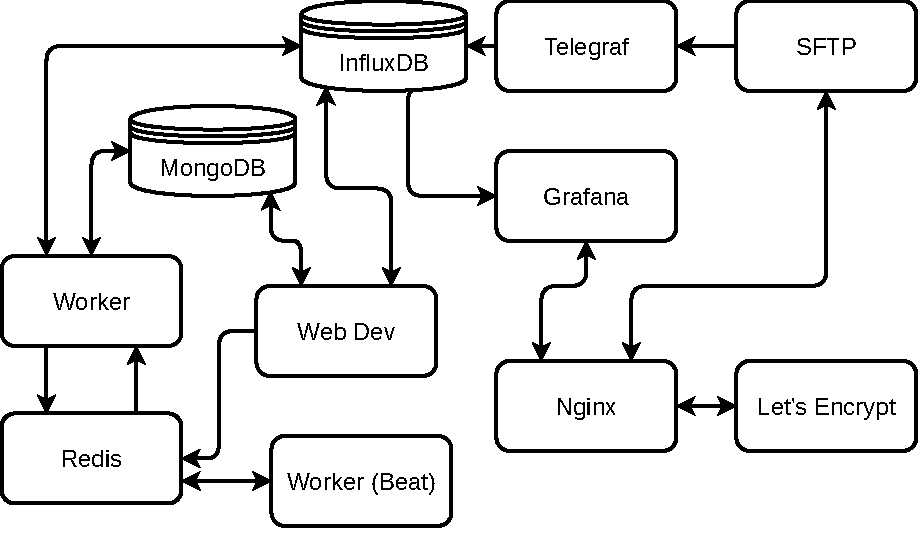
\includegraphics[width=0.90\textwidth]{img/diagrams/pdf/old-arch-connections.drawio.pdf}
    \caption[old-arch-connections listing]{old-arch-connections caption under figure}
    \label{fig:old-arch-connections}
\end{figure}




Each \gls{ec2} instance runs a Docker container for each one of the following services:
 
\begin{itemize} 

\item \textbf{InfluxDB\footnote{https://www.influxdata.com/products/influxdb-overview/}\label{foot:influxdb}} (Timeseries Database)
\item \textbf{Telegraf\footnote{https://www.influxdata.com/time-series-platform/telegraf/}\label{foot:telegraf}} (Data collecting service)
\item \textbf{MongoDB\footnote{https://www.mongodb.com/}\label{foot:mongodb}} (General use, no-SQL, Document Database)
\item \textbf{Grafana\footnote{https://grafana.com/}\label{foot:grafana}} (Web platform for data visualization, the front end of the \gls{dss})
\item \textbf{Nginx\footnote{https://www.nginx.com/}\label{foot:nginx}} (Reverse proxy with \gls{https} capabilities)
\item \textbf{Let's Encrypt\footnote{https://letsencrypt.org/}\label{foot:letsencrypt}} (Automatic \gls{tls} Certificate installer, companion for the Nginx container)
\item \textbf{Web Dev} (Flask\footnote{https://flask.palletsprojects.com/en/2.1.x/}\label{foot:flask} Web platform / API for managing Workers' settings)
\item \textbf{Redis\footnote{https://redis.io/}\label{foot:redis}} (Message Queue System for queuing Worker's jobs)
\item \textbf{OpenSSH\footnote{https://www.openssh.com/}\label{foot:openssh}} (\textit{atmoz/sftp}) (\gls{ssh} Server for receiving client data through \gls{sftp})
\item \textbf{Workers} (Celery\footnote{https://docs.celeryq.dev/en/stable/}\label{foot:celery} Container running the Forecast, Simulation and Optimization \textit{Python} Algorithms as well as the \gls{kpi} Algorithms.)
\item \textbf{Workers} (\textit{Beat}) (Celery Container that periodically \textit{triggers} jobs in the Workers container)

\end{itemize}


\subsubsection{Service's Connections}

In \Cref{fig:old-arch-connections} the relations between these containers can be schematically seen. Starting on the right side, with the  Let's Encrypt and Nginx containers, these provide outside access to the Grafana and SFTP services inside the respective containers. Data from the InfluxDB database is read by the Grafana service which allows the Client's users and the company's developers to query the database and at the same time generate charts with such information. Client sensor data is sent to the SFTP server that shares the incoming files with the Telegraf service and allows it to pre-process that sensor data and proceed to the data intake into the InfluxDB database. Then, either through remote access to the Web Dev container or automatically through the Worker Beat service, tasks are sent to the celery queue (using the Redis service) and picked up by the Worker service. This Worker service then accesses the MongoDB Database to load algorithm and device configurations and the required client sensor data from the InfluxDB database before running the tasked algorithm. Data resulting from the execution of the algorithms is then sent to the InfluxDB database, to be read by the Grafana service. There are some connections that are bidirectional, such as the Web Dev to the MongoDB database which is the service used to manipulate the MongoDB database's algorithm and device configurations.


\subsubsection{Databases}\label{methodology:sss:databases}

There are two types of databases being used by this architecture: A Timeseries Database, in this case \textbf{InfluxDB}, and an additional general-purpose Document Database: \textbf{MongoDB}. Each type of database has a different role, the first one stores the Client's timeseries data such as sensor information, pump orders, predicted tank levels, etc.
The second one, the Document Database, is responsible for storing configuration settings for each worker service (optimization, simulation and forecasting), for storing electrical tariffs data and to store sensor device's configurations.

\subsubsection{Grafana}\label{methodology:sss:grafana}

This web platform allows the visualization of the Timeseries data from the \textbf{InfluxDB} database. This is an open-source platform that runs on a docker container with little to no modifications necessary. The dashboards are built using the built-in tools and allow for complex and very informative data visualization. 

\subsubsection{Telegraf}\label{methodology:sss:telegraf}

The \textbf{Telegraf} container is used to gather the files containing the raw sensor data sent from the Client to the \gls{sftp} server. Since this container shares the file upload location folder with the \gls{sftp}, through a convoluted process of storing the filename of the last file uploaded, periodically checking for the next file and file handling \textit{spaghetti} code that spans multiple files and has an enormous codebase that weighs the docker image's file size considerably. 

\subsubsection{\gls{sftp}}\label{methodology:sss:sftp}

The \gls{sftp} service here provides a secure method for the Clients to send files containing the Timeseries data to our servers, where they can be processed and turned into actionable insights by the algorithms running in the Workers container. The Client sends their public key (from a cryptographic key pair) when the project start to authenticate against this \gls{sftp} service and uploads the files to a pre-designated folder. These files are then accessed by the Telegraf container which performs the file intake process.


\subsubsection{Nginx + Let's Encrypt}\label{methodology:sss:nginxletsencrypt}

These two containers allow secure Internet access from the \gls{ec2} instance into the correct docker container IP address and port. The Client-facing services Grafana and \gls{sftp} which, respectively, provide the web interface for the \gls{dss} and client file input service are inside containers which themselves can change their internal IP inside the Docker environment. To keep the dynamic IPs in check and allow for these services to be accessed from outside the Docker environment, the Nginx container keeps track of this dynamic IP and updates its route table accordingly. This allows for any of these two containers to restart, change their IP address and still not break the routing back to the host \gls{ec2} instance, which has an \gls{eni} associated to it exclusively. This \gls{eni} is then connected, exclusively, to a single \gls{eip} to which the Clients connect, like \Cref{fig:old-arch-nginx} implies.

As for the Let's Encrypt container, this container shares a docker volume with the Nginx container and automatically and periodically maintains the \gls{tls} certificate files that the Nginx requires in order to serve the Grafana interface through \gls{https}. 
\begin{figure}[!htbp]
    \centering
    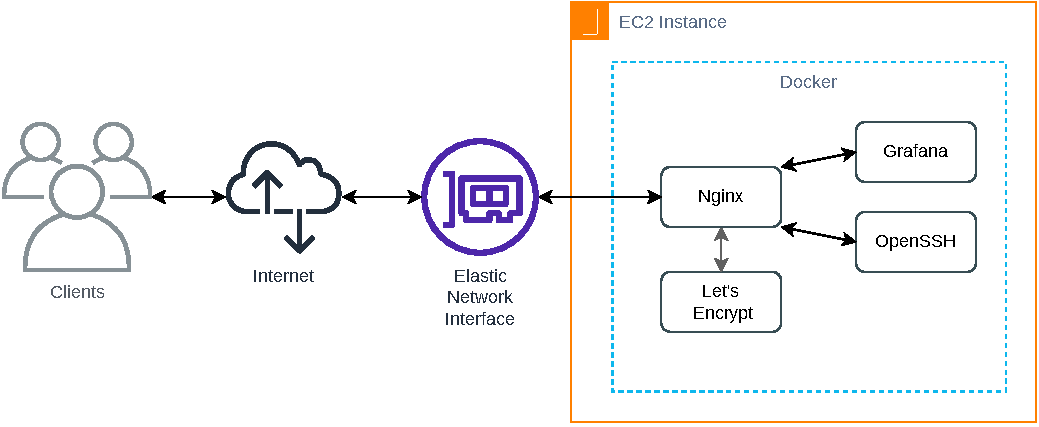
\includegraphics[width=0.90\textwidth]{img/diagrams/pdf/old-arch-nginx.drawio.pdf}
    \caption[Internet access to the Client-facing services]{Internet access to the Client-facing services.}
    \label{fig:old-arch-nginx}
\end{figure}


\subsubsection{Redis}\label{methodology:sss:redis}

Redis is used as a message queue backend for Celery, enabling other services to send Celery tasks to a queue for asynchronous execution by the Workers.

\subsubsection{Web Dev}\label{methodology:sss:webdev}

Based on Flask, this web application serves an \gls{api} as well as serving a web page that gives developers access to algorithm configurations and the ability to push Celery tasks to the queue. This application connects directly to both databases.

\subsubsection{Workers}\label{methodology:sss:workers}

The Workers' container image is built \textit{in-house} by the development team, using a \textit{Python} Docker image as the base image, wherein all the company's algorithms lay. The \textit{forecast}, \textit{optimization} and \textit{performance analysis}/\gls{kpi} algorithms are individually linked in a Celery configuration file, which defines how each algorithm is executed in a Celery task and how that task is called. This container executes a Celery Worker that executes all Celery Tasks in the Celery task queue.

When a task is sent to the task queue, this Celery Worker who polls the task queue, picks the task up and starts executing the task as soon as possible.

There are two Workers images, the first one contains the code for all algorithms and is the one which starts the Celery worker. The other one, which is internally called Celery Beat, executes a Celery instance in \textit{Beat} mode which sends pre-configured Celery tasks to the queue. This is used to run the algorithms periodically in order to process the Client data and generate actionable insights for the Client.

These algorithms require decent amounts of computer resources, namely CPU power and RAM capacity, in order to be able to run effectively. This is a direct contrast to the remaining components of this old architecture, which see minimal Client use and are therefore less resource intensive. In terms of storage, the situation is the opposite since these algorithms use data stored within the other services: the database services.

\subsection{Issues}\label{methodology:ss:Issues}


Besides an individual \gls{ec2} instance, each Client also has an individual GitLab\footnote{https://gitlab.com/}\label{foot:gitlab} project, which is composed of several, and different Git\footnote{https://git-scm.com/}\label{foot:git} code repositories. Each GitLab project contains the following repositories:

\begin{itemize}

    \item \textbf{dbs} (Databases configurations, build files for databases' docker images, deployment scripts)
    \item \textbf{Workers} (Build files for the Workers' docker images)
    \item \textbf{DBconnectors} (Standardized code for database access)
    \item \textbf{forecast\_optimization\_api} (Code and build files for the Web Dev docker image)
    
\end{itemize}

In the \textbf{dbs} repository, build scripts for custom docker images for InfluxDB, Nginx and Telegraf can be found. Also, here reside the scripts that are used to remotely deploy docker containers to the \gls{ec2} instances as well as the \textit{docker-compose} configuration files. The GitLab \gls{cicd} pipeline that deploys the old architecture to the instances also resides here.

As for the \textbf{DBconnectors} repository, database connectors can be found. These allow offloading the code that connects to the databases from the algorithms to a separate module, which can be reused throughout the same GitLab Project and, in theory, keep the query methods consistent for both the \textbf{Workers} and \textbf{Web Dev} codebases.

In the \textbf{Workers} repository, the code for the algorithms used by the platform to perform the forecasting, optimization and KPI calculation as well as the \textbf{DBconnectors} repository linked as a submodule can be found.

In the likeness of the \textbf{Workers} repository, the \textbf{forecast\_optimization\_api} repository also imports the \textbf{DBconnectors} repository as a submodule. This \textbf{forecast\_optimization\_api} repository is where the \textit{Web Dev} container build code is situated. 

\subsubsection{Low Cohesion and High Coupling}\label{methodology:sss:low-cohesion-and-high-coupling}

This old architecture has severe problems regarding its Cohesion and Coupling.

The readers notice that, as shown both above and on \Cref{fig:old-arch-connections}, there are multiple services performing read and write operations to the InfluxDB database. Although concurrency is not a major problem, having different schemas and tag names for InfluxDB queries in different services has historically led to multiple timeseries data not being detected when querying the database when a different querying service placed the data in the database. This is due to mismanagement of repositories and git submodules, and requires additional care, planning and communication from the developer team's side. Here, having a specific service to perform pre-prepared queries, with very detailed database schemas, to which all other services would connect to query/write to the database would solve this problem. Here, cohesion is low, since code that is used to connect to the database is spread out throughout the codebase. It also means that there is \textit{major implementation coupling}.

Then, there are issues regarding \textit{temporal coupling}. When performing data intake, the timeseries database, the data intake service(Telegraf), the SFTP service and the Nginx service all need to be up and running and accessible to be able to perform data intake. If one of these services is unavailable, data that is sent from the Client is not processed when the unavailable service becomes available again. This has been something that has happened before, with some regularity, and the only way to recover the missing data is through manual data intake of the received text or sheet files that are sent to the SFTP service which is tedious and prone to errors.

Finally, there is the issue of \textit{deployment coupling}. In order to deploy a small change to any of the services, all docker containers are shutdown and restarted, which results in considerable \textit{downtime} for each Client.


\subsection{Replaceability}\label{methodology:sss:replaceability}

The old architecture possesses low replaceability, since it's not easy to change a service for another, such as the timeseries database or the data intake service. For example, with the exception of the data visualization service (Grafana), major refactoring of code would have to be done, since each service connects to the timeseries database in different ways, independently.

\subsection{Resiliency}\label{methodology:sss:resiliency}

Despite the high coupling of the application, with the old architecture using docker containers, usually the application doesn't become totally unusable if one of the service fails. The problem lies with the docker orchestrator or the EC2 instance itself. If one of these fail, then the whole application becomes instantly unavailable. If the EC2 instance becomes unresponsive, as has happened multiple times before, then a manual, full system reboot of the instance followed by a redeployment of the whole application stack is inevitable. 

\subsection{Deployments}\label{methodology:sss:deployments}

A deployment of the application that uses the old architecture is a tiresome and arduous affair, since the application is highly deployment coupled as stated before. After \textit{committing} a change to one of the repositories, Deployment involves \textit{tagging} the repository of code in which the change was made in order to create the necessary docker images with those tags through \gls{cicd}. In this step, a GitLab runner will pull the repository, checkout any git submodules, perform unit tests, and then start building a docker image with the code inside the whole repository. Currently, for the old architecture, this step takes around 10 minutes to complete. After the tagging of the repository of code is done, the next step is to perform the same task with the \textit{dbs} repository, where another 10 to 20 minutes of docker image building takes place. Then, after all of the docker images are built, the GitLab runner open an SSH shell to the EC2 machine of the Client, pulls the respectively tagged docker images and performs a docker-compose operation. This operation instructs the docker orchestrator to shut down all running containers, delete the volumes (with the exception of the databases) and then re-create the containers with the newer docker images. In all, this process takes around 30 minutes to complete. During this last step, the Users experience \textit{downtime} with a duration of between 1 and 4 minutes, if the deployment is successful.

If a change is to be done for all Clients simultaneously, this process needs to be repeated individually, once for each client. 

\subsection{Testing}\label{methodology:sss:testing}

Having the components of the application so tightly coupled, means that it requires the entire application to be executed in order to properly test the entire application. This is cumbersome and forces the developers to have a local copy of the entire application, including the timeseries data. This data can have big dimensions, and the only method to test with this data is to execute a script that connects remotely through SSH to the EC2 machine and makes a copy of the timeseries' docker instance's volume. Said volume copy is then transferred back to the developer through an SSH tunnel, so that the developer can then use that volume with the timeseries' docker instance that is running locally, for testing. Besides the massive data copy, which occupies disk space in the developers' computer and results in higher data transfer costs in the AWS account, the developer is required to have hardware capable of loading and executing all services simultaneously.

\subsection{Scaling}\label{methodology:sss:scaling}
\textcolor{orange}{ Needs re-read and possible refactoring}

The contrast between the different services' computational and storage requirements is one of the major issues of the old architecture. Adequate instance sizing is essential to lower infrastructure costs with compute resources. As can be seen in \Cref{fig:caesb-cpu-usage}, the CPU average utilization is usually very low, indicating that the resources allocated to this instance are way overestimated, elevating the infrastructure costs for no reason. However, the peaks in CPU usage that can be observed in this same Figure, which are caused by the periodically-running algorithms, push this CPU usage up to levels that suggest the allocated resources are somewhat adequate for this use-case. And wherein lies one of the major issues: over a 24-hour period, the amount of time spent with very low CPU usage is visibly and significantly superior to the time spent with adequate CPU usage for the instance size. 

\begin{figure}[!htbp]
    \centering
    \fbox{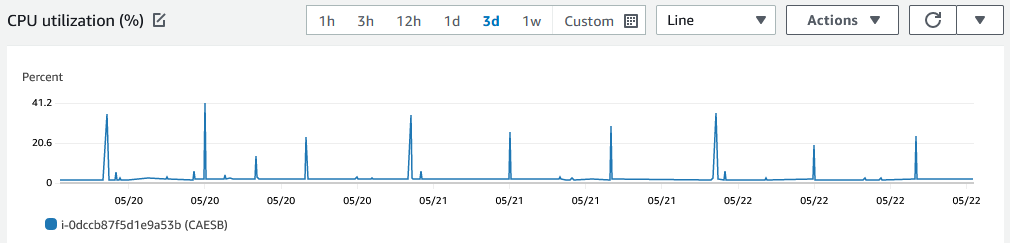
\includegraphics[width=0.95\textwidth]{img/screenshots/caesb-cpu-usage.png}}
    \caption[Client CPU Usage Example]{Client's \gls{ec2} Instance average CPU usage, during a three-day period, in 5 minutes intervals.}
    \label{fig:caesb-cpu-usage}
\end{figure}
    

The \gls{ec2} instance upon which these services reside can be provisioned and sized to different computational and storage needs. However, this would mean that it would either be adequately sized for the times the workers are dormant and undersized for when the worker's algorithms are running, or oversized for most of the time and only adequately sized while running said algorithms. Unfortunately, resizing an \gls{ec2} instance requires downtime for the whole platform, since it requires the \gls{ec2} instance to be rebooted. Since this would also stop Client access to the \gls{dss} and data intake service, this option cannot be contemplated. After testing a platform implementation with an instance adequately sized for the instants when workers are dormant, it was concluded that the algorithms would either refuse to run or crash when performing resource intensive calculations due to low RAM availability. The decision was then made, to keep the platform running in oversized, and costly, \gls{ec2} instances.

Therefore, one of the goals of this work is to attempt to solve this problem. One of the possible general solution was to split the resources based on their compute resource requirements. Having the workers on a separate \gls{ec2} instance that would be automatically and periodically provisioned and unprovisioned according to a schedule would allow the remaining services to be placed in a lower cost \gls{ec2} instance, lowering the overall infrastructure costs. However, without altering the existing architecture, this would mean that the alteration would only be the place where the Workers' docker container would be executed. Since the amount of \gls{ec2} instances is directly proportional to the amount of Clients, having two instances would duplicate the computational resources, networks connections and storage space needed to maintain the platform for all Clients. This would exacerbate the problem of limited compute resources available to our \gls{aws} account.

%\subsection{Limited Compute Resources}\label{methodology:ss:limited-compute-resources}

One of the issues with the old architecture is that the number of \gls{ec2} instances needed was directly tied to the amount of Clients, since each Client required its own instance to host the platform, generating what is called a Scalability problem. For the company's \gls{aws} account, a limit of thirty-two (32) \gls{vcpu} units (each \gls{vcpu} corresponds to a processing thread in a CPU core) was imposed by Amazon as default, which meant that the sum of \gls{ec2} instance's \gls{vcpu} units could not surpass this value. Each client requires an \gls{ec2} instance of the type \textit{t3a.large} or \textit{t3a.xlarge}, respectively two (2) or four (4) \gls{vcpu} units, depending on the Client's Water Network's size and complexity and contracted services. This would mean that the amount of clients was limited from sixteen (16) clients if they all used the smaller instance or down to eight (8) clients if these Clients required more resources. As can be concluded, this is a hard limit on the amount of clients that can be served simultaneously by the company, which is an obvious problem.


\subsection{Cost-Effectiveness}\label{methodology:sss:cost-effectiveness}
\textcolor{orange}{ Discuss how the old arch is costly and not very efficient at it}

\subsection{FKMs}\label{methodology:sss:fkms}

Regarding the \gls{fkm}, based on the previous issues that have been shown, by using the old architecture, the development team has suboptimal results in the metrics.

As mentioned in \cref{methodology:sss:deployments}, the difficulty with which deployments are performed forces the development team to gather numerous changes before deploying them so that the deployment can be performed less frequently, resulting in less \textit{downtime} for the client. This, inevitably, lead to both a lower \textit{Deployment Frequency} and also a bigger \textit{Lead Time for Change}.

In \cref{methodology:sss:deployments}, it's also mentioned the amount of \textit{downtime} that is to be expected when deploying changes to production. Such an amount of \textit{downtime} is unacceptable for a normal, eventless deployment. However, when failure occurs in the application using the old architecture, the \textit{Time to Restore Service} is composed of multiple amounts of time: the time it takes for the failure to be detected, the time is takes to find a mitigation for the failure or troubleshooting time, the time it takes to re-deploy the application (which is around 20 to 30 minutes in case the mitigation requires changes to the code) and the time it takes for the recently deployed services to be back online. If failure occurs during the run of a task, that task (and subsequent tasks that failed to start) will need to be run manually as well. 

Since the development team gathers numerous changes before deploying them to production, the chance of failure increases. Besides exacerbating the problem with the \textit{Time to Restore Service}, this method of deployment also increases \textit{Change Failure Rate}.



\subsection{Observability}\label{methodology:ss:observability}

One of the issues with the old architecture was the lower Observability that it provided to the Maintainers. Despite having extensive logging for each one of the services, the other two key components of Observability - metrics and tracing - were not present at any meaningful scale. Having to peruse hundreds of lines of code, filtering different services and log levels just to manually create metrics for algorithm execution time was time-consuming and tiresome. There was also no tracing put into place anywhere in the platform. To combat this, it was stipulated by the \textit{stakeholders} that the new architecture should contemplate measures to increase observability of the entire system.

\subsubsection{Alerts}\label{methodology:sss:alerts}
A consequence of the old architecture's lack of system observability, there were no useful metrics being created and store besides the ones pertaining to the algorithm result. Metrics are required in order to, having a set of thresholds for each one of them, produce alarms. Alarms automatically inform the Maintainers and \textit{stakeholders} of unexpected system behavior or catastrophic system failure in a timely manner, giving the chance for the development team to trace the cause(s) of the problem(s) before they become apparent and/or disruptive to the Clients. For some Clients, there were metrics and alarms setup based on the Tank's water level that would send messages to a Slack channel shared between the company and the respective Client, but fell into disuse.

\subsubsection{Singular Environment}\label{methodology:sss:singular-environment}

One of the faults with the older architecture was the lack of different environments for deployment. Such fact meant that every deployment made to each Client had the very real possibility of breaking Production for that particular Client, where the faults would impact the Client's usage of the platform directly. This was a recurring event when deploying, as the algorithms are quite complex. Given the fact that some algorithms use real-time data gathered from the last one hundred (100) days, the somewhat unpredictable nature of the algorithms' execution results made the repeatability of results from day to day not trivial.
Breaking changes were also not always apparent, since some algorithms performed calculations using data generated by other algorithms and/or real-time data and such mistakes only became apparent on the following work day, after their execution. There were cases when the algorithms ran perfectly during week days, but failed during the weekends (since the water consumption patterns change accordingly).

All of these mishaps lead to the creation of a staging server where changes to the platform or algorithms could be tested with real data, causing no impact to the Clients and allowing for results to be monitored for longer periods of time to ascertain system reliability. As such, a staging environment should replicate as much as possible the production environment, be it the Operating System version, it's installed packages, \textit{Python} versions, \textit{Python} packages, the data in the server, the quick-fixes applied to production, etc.
This, however, meant that a similar, staging environment \gls{ec2} instance needed to be running simultaneously with the production environment's \gls{ec2} instance, effectively doubling the infrastructure costs. Since each Client had its own \gls{ec2} instance, this approach would also be impossible to maintain. An attempted approach was to use a single \gls{ec2} machine, sized similarly to the highest performing \gls{ec2} machine used by one of the Clients, to act as a staging server for each Client at a time. Each time a major change was to be deployed to a Client, it would be first deployed during a set time to this staging server and upon success, be deployed to the Client's production server. Having multiple developers perform different deployments, for different Clients, at the same time, meant that Deployment Frequency lowered and Lead Time for Change increased as well.


\section{Proposed New Architecture}\label{methodology:s:proposed-new-architecture}

``The primary measure of success of a software system is the
degree to which it meets the purpose for which it was
intended''

\textcolor{orange}{Small intro to the new architecture}

\textcolor{orange}{The next part will also be refactored:}

Changing from the old architecture to the new one isn't a straightforward process. Having clients who are still using the infrastructure upon which the old architecture relies doesn't allow for mistakes while doing the migration. This would bring several challenges, which were compounded by the lack of a functional new web interface for the new architecture. For this migration to occur, careful planning had to be done and checked by the \textit{stakeholders} before any changes were put into production. Measures such as changing network configurations, restarting services or run benchmarks on the old infrastructure could not affect any Clients using the old infrastructure.

To further complicate the planned migration, during the planning and implementation phase of this project the \textit{stakeholders} required multiple changes to accommodate new Clients, which had to be applied to the new architecture. These changes and late-requests shaped the decisions taken during the planning and implementation phase of the migration. For one of the new Clients, that the \textit{stakeholders} arranged while the migration was concurring, there was a dilemma: Further increase the number of Clients using the old architecture (and subsequently, old infrastructure) or risk having this new Client as test subject for the new architecture? After discussion with the \textit{stakeholders}, the development efforts were shifted from all current project to implementing the new architecture and adapting the algorithms to make use of this new architecture and 


\subsection{Overview}\label{methodology:ss:overview-new-arch}
Based on the recently elicited requirements and the issues with the old architecture, a generic plan for the new architecture is defined as follows on \Cref{fig:new-arch-basic}

\begin{figure}[!htbp]
    \centering
    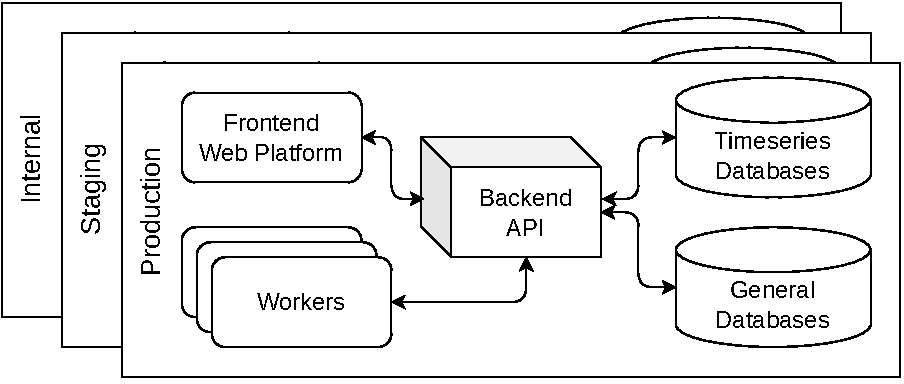
\includegraphics[width=0.90\textwidth]{img/diagrams/pdf/new-arch-basic.drawio.pdf}
    \caption[new-arch-basic listing]{new-arch-basic caption under figure}
    \label{fig:new-arch-basic}
\end{figure}



\subsection{New components}\label{methodology:ss:new-components-new-arch}

\subsubsection{Serverless}\label{methodology:sss:serverless}


\subsubsection{Backend API}\label{methodology:sss:backendapi}
The first element of the new architecture to be researched and produced was the Backend \gls{api}. A new \gls{api} solves the problem that existed with having different methods to read and write to the databases. Using this Backend \gls{api}, each service that requires access to the database is therefore required to have authorization to access the Backend \gls{api}, which in turn reinforces security regarding database access. Having a standardized method to access the databases also allows for easier debugging, since every service uses the same\gls{api}interfaces, which can help rule out databases and the Backend\gls{api}from possible fault causes.

The old architecture had a Flask \gls{api} that served a webservice through which developers could manually tweak optimization and forecasting settings and issue tasks. This api, however, had no security features nor any authentication in place, with its access limited only through network settings, where each developer had to manually establish an \gls{ssh} tunnel to the Client's \gls{ec2} machine in order to access said api. Due to time constraints and limited knowledge inside the company regarding securing a Flask api, research had to be performed in order to determine the best course of action regarding the choice of web framework for a Backend API.

\subsection{((fixes))}\label{methodology:ss:fixes}
\textcolor{orange}{How the new architecture solves the issues with the old architecture}



\textcolor{red}{The rest of the text is to be removed/relocated/refactored so much that I don't even know if or where to place it}



\subsection{\textit{Stakeholders}}\label{methodology:s:stakeholders}

The first step when handling a Software Engineering problem is to identify the key \textit{stakeholders}. For this project, the key stakeholders are all the people involved in the company and the Clients' project managers. In the company, SCUBIC, the teams are divided into the development team, the executive team and the operations team, where their members are part of one or more of them.